\documentclass[11pt,]{article}
\usepackage{lmodern}
\usepackage{amssymb,amsmath}
\usepackage{ifxetex,ifluatex}
\usepackage{fixltx2e} % provides \textsubscript
\ifnum 0\ifxetex 1\fi\ifluatex 1\fi=0 % if pdftex
  \usepackage[T1]{fontenc}
  \usepackage[utf8]{inputenc}
\else % if luatex or xelatex
  \ifxetex
    \usepackage{mathspec}
  \else
    \usepackage{fontspec}
  \fi
  \defaultfontfeatures{Ligatures=TeX,Scale=MatchLowercase}
\fi
% use upquote if available, for straight quotes in verbatim environments
\IfFileExists{upquote.sty}{\usepackage{upquote}}{}
% use microtype if available
\IfFileExists{microtype.sty}{%
\usepackage{microtype}
\UseMicrotypeSet[protrusion]{basicmath} % disable protrusion for tt fonts
}{}
\usepackage[margin=1in]{geometry}
\usepackage{hyperref}
\hypersetup{unicode=true,
            pdftitle={Cartogram Mapping and its Application to Cancer Data Visualisation},
            pdfauthor={Stephanie Kobakian, Jessie Roberts and Dianne Cook},
            pdfborder={0 0 0},
            breaklinks=true}
\urlstyle{same}  % don't use monospace font for urls
\usepackage{longtable,booktabs}
\usepackage{graphicx,grffile}
\makeatletter
\def\maxwidth{\ifdim\Gin@nat@width>\linewidth\linewidth\else\Gin@nat@width\fi}
\def\maxheight{\ifdim\Gin@nat@height>\textheight\textheight\else\Gin@nat@height\fi}
\makeatother
% Scale images if necessary, so that they will not overflow the page
% margins by default, and it is still possible to overwrite the defaults
% using explicit options in \includegraphics[width, height, ...]{}
\setkeys{Gin}{width=\maxwidth,height=\maxheight,keepaspectratio}
\IfFileExists{parskip.sty}{%
\usepackage{parskip}
}{% else
\setlength{\parindent}{0pt}
\setlength{\parskip}{6pt plus 2pt minus 1pt}
}
\setlength{\emergencystretch}{3em}  % prevent overfull lines
\providecommand{\tightlist}{%
  \setlength{\itemsep}{0pt}\setlength{\parskip}{0pt}}
\setcounter{secnumdepth}{5}
% Redefines (sub)paragraphs to behave more like sections
\ifx\paragraph\undefined\else
\let\oldparagraph\paragraph
\renewcommand{\paragraph}[1]{\oldparagraph{#1}\mbox{}}
\fi
\ifx\subparagraph\undefined\else
\let\oldsubparagraph\subparagraph
\renewcommand{\subparagraph}[1]{\oldsubparagraph{#1}\mbox{}}
\fi

%%% Use protect on footnotes to avoid problems with footnotes in titles
\let\rmarkdownfootnote\footnote%
\def\footnote{\protect\rmarkdownfootnote}

%%% Change title format to be more compact
\usepackage{titling}

% Create subtitle command for use in maketitle
\providecommand{\subtitle}[1]{
  \posttitle{
    \begin{center}\large#1\end{center}
    }
}

\setlength{\droptitle}{-2em}

  \title{Cartogram Mapping and its Application to Cancer Data Visualisation}
    \pretitle{\vspace{\droptitle}\centering\huge}
  \posttitle{\par}
    \author{Stephanie Kobakian, Jessie Roberts and Dianne Cook}
    \preauthor{\centering\large\emph}
  \postauthor{\par}
    \date{}
    \predate{}\postdate{}
  

\begin{document}
\maketitle

{
\setcounter{tocdepth}{2}
\tableofcontents
}
\section*{Abstract}

\hypertarget{introduction}{%
\section{Introduction}\label{introduction}}

Maps have been adopted to present geospatial statistics for centuries.
Maps connect data and statistics to the geographical representation of
areas that are generally familiar to the audience. However, it is not
enough for areas on maps to be recognisable, if information regarding
the distribution of the statistic cannot be gleaned. In situations where
the people are of interest, not the land they live on, it is reasonable
to explore views that enhance the communication of the cancer
statistics. Identifying and explaining spatial structures, patterns, and
processes involves considering the individuals in communities and
organising communities into representable units (Moore and Carpenter
\protect\hyperlink{ref-SAMGIS}{1999}). This has spurred innovations over
the previous centuries to enhance the shapes and maps presented to
effectively communicate cancer outcomes, and health outcomes more
broadly. Cancer statistics directly represent and relate to the people
living within individual geographical areas.

The visualisation methods used to present cancer statistics will depend
on the intended message and users of the map. Transforming statistics to
visualisations considers individual observations or observation points
aggregated into communities and geographical units. Visualising diseases
on maps is often the first step in exploratory spatial data analysis and
effectively helps in the formulation of hypotheses (Jahan et al.
\protect\hyperlink{ref-MTMSIH}{2018}). Disease maps help to present
geographic patterns that may have been overlooked in a table, obscuring
the geospatially related statistics (Moore and Carpenter
\protect\hyperlink{ref-SAMGIS}{1999}). By providing a visual
representation of cancer outcomes, geographic patterns of disease are
able to be identified and effectively addressed.

\hypertarget{disease-mapping-methods}{%
\section{Disease mapping methods}\label{disease-mapping-methods}}

\hypertarget{current-best-practice-map-displays-for-cancer-data}{%
\subsection{Current best practice map displays for cancer
data}\label{current-best-practice-map-displays-for-cancer-data}}

A choropleth map is used to display the spatial characteritics of a
relationship, or variability, of measurements. As an alternative storage
device to a table, it preserves locations for geographically ordered
data, with usage dating back to the 1800s (Berry, Morrill, and Tobler,
\protect\hyperlink{ref-GOINO}{n.d.}). A choropleth is constructed by
drawing the geographic or political boundaries, and filling the shapes
with colours to represent values of a measured variable (Tufte
\protect\hyperlink{ref-EI}{1990}). Early versions of choropleth maps
used symbols or patterns instead of colour. Bell et al.
(\protect\hyperlink{ref-CPISACA}{2006}) discusses their use in
visualising cancer data, and Walter
(\protect\hyperlink{ref-DMAHP}{2001}) gives an overview of the
development of these maps for displaying disease data. Just as
geographers are no longer the only creators of maps, Bell et al.
(\protect\hyperlink{ref-CPISACA}{2006}) suggests the audiences of
spatial health data analysis have extended beyond researchers to the
public, policymakers and the media. A choropleth map is a true map of
the topology, constructed for visual inspection of spatial patterns
across a familiar geographic form. Figure 1 shows a choropleth map where
each state of the United States of America is coloured by the average
annual rate of new cases of lung and bronchus cancer from years 2012 to
2016.

\begin{figure}

{\centering 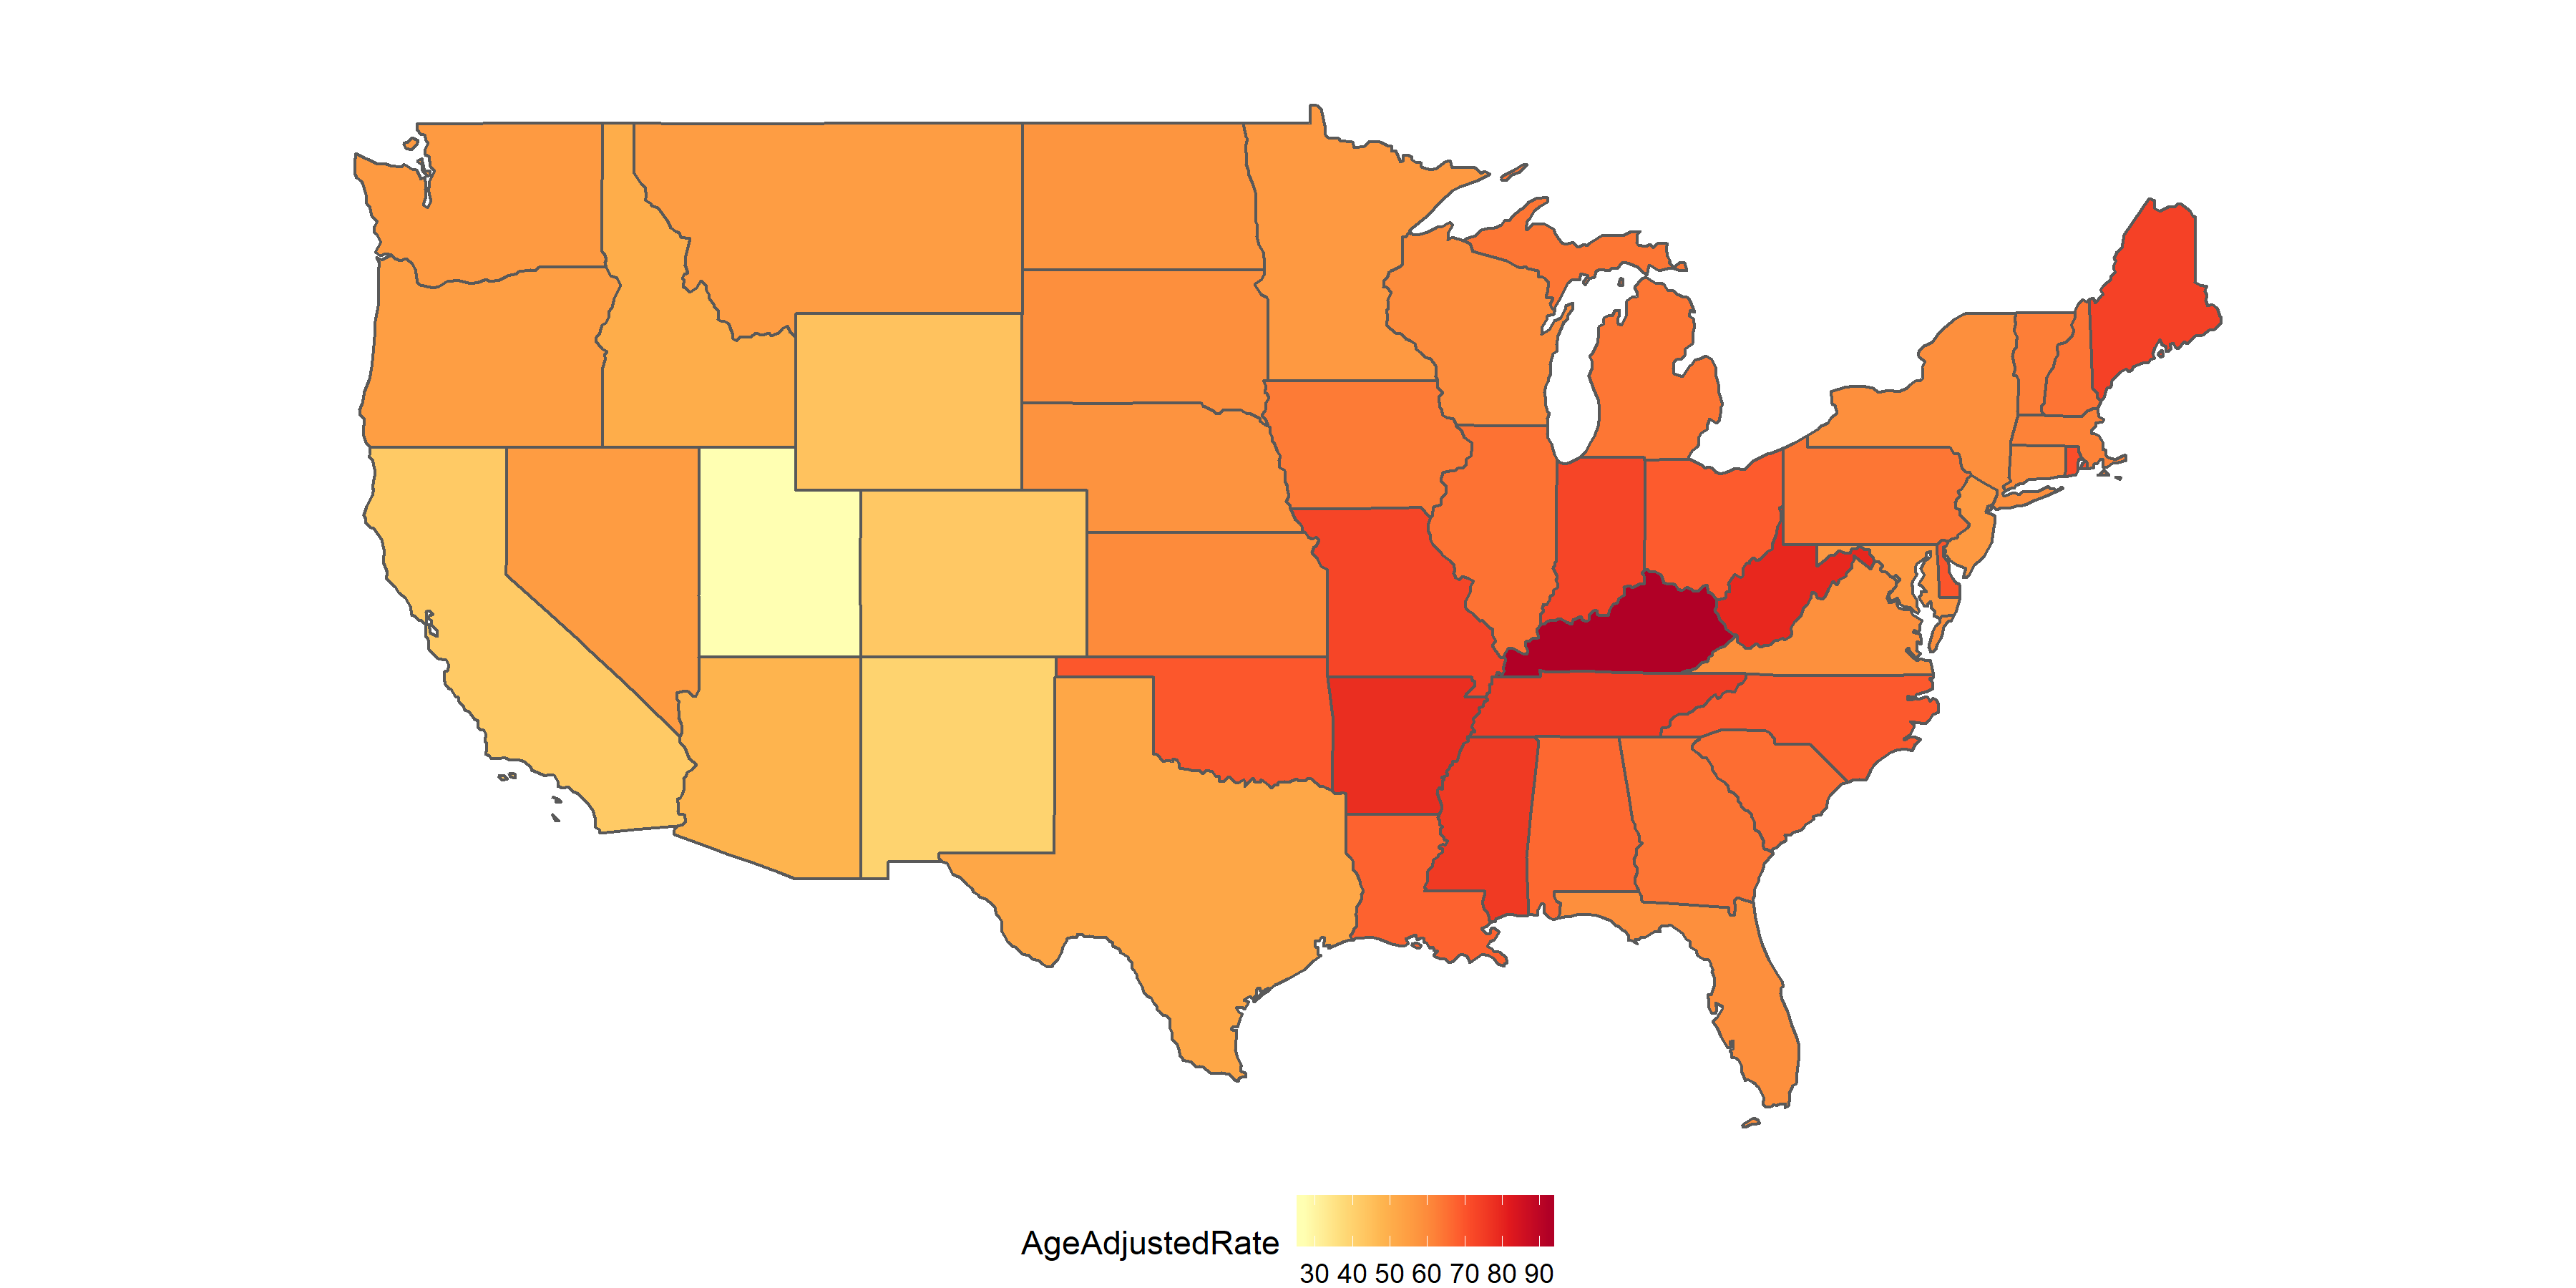
\includegraphics[width=0.8\linewidth]{figures/ggchoro} 

}

\caption{A choropleth map of the United States of America.}\label{fig:choro}
\end{figure}

Utilising the familiar state boundaries can make a map intuitive to read
(Brewster and Subramanian \protect\hyperlink{ref-CIBMUK}{2010}), and
allow viewers to visually infer the spatial relationships in the data,
i.e.~how cancer rate differs across the states. The familiarity of the
geography is a worthy consideration when presenting results of spatial
analysis. Just as geographers are no longer the only creators of maps,
Bell et al. (\protect\hyperlink{ref-CPISACA}{2006}) suggests the
audiences of spatial health data analysis have extended beyond
researchers to the public, policymakers and the media. While the areas
are recognisable shapes, they are often politically driven boundaries
with individual areas being of non-uniform size, containing different
population densities and subject to change over time. The different
population and geographical sizes of administrative areas can attract
attention to the shades of the unpopulated but large areas (Tufte
\protect\hyperlink{ref-EI}{1990}). Choropleths can inhibit visual
inference when presenting human related statistics as the display may
draw attention from the `potentially more important results in the more
populous communities' (Exeter \protect\hyperlink{ref-SE}{2017}).

Choropleth maps can be useful devices for communicating information to
public on a familiar map base. In epidemiology, choropleths are often
used as a tool to study the spatial distribution of cancer incidence and
mortality. A cancer atlas is a choropleth map, or collection of maps,
representing cancer incidence and mortality for a country, or group of
countries. d'Onofrio et al. (\protect\hyperlink{ref-MACM}{2016}) provide
the definition and reports that cancer atlases began with Haviland's
maps in 1875. The data collection methods of cancer mortality rates
across regions, and the administrative control within regions lends
itself to choropleth visualisation. The increasing development and use
of disease maps can be attributed to the availability of geographic
information system software (Exeter \protect\hyperlink{ref-SE}{2017}).
Early work in US cancer atlases can be attributed to Burbank ???, and UK
cancer atlases to Howe 1963 ???. The choropleth maps presented levels
via hatchings or dots on a black and white scale. These atlases were key
to developing hypotheses regarding areas with unusually high rates,
geographic correlations, work related exposures, and high risk diets
d'Onofrio et al. (\protect\hyperlink{ref-MACM}{2016}).

Almost 100 years of cancer mapping in the United States and the United
Kingdom has seen increased effectiveness in the presentation cancer
statistics. Mortality rates are now often presented as relative rates of
risk across the population, and age adjusted to correct for the the
higher prevalence of cancers in older populations. Howe
(\protect\hyperlink{ref-HEDP}{1989}) describes Stock's development of
the standardised mortality ratios through the 1930s. Table 1 presents
summarises the measures presented in published cancer atlases, and
provides a definition of each measure.

Table 1: Measures used to report cancer statistics

\begin{longtable}[]{@{}ll@{}}
\toprule
\begin{minipage}[b]{0.28\columnwidth}\raggedright
Measure\strut
\end{minipage} & \begin{minipage}[b]{0.66\columnwidth}\raggedright
Details\strut
\end{minipage}\tabularnewline
\midrule
\endhead
\begin{minipage}[t]{0.28\columnwidth}\raggedright
1. IR (Incidence Ratio)\strut
\end{minipage} & \begin{minipage}[t]{0.66\columnwidth}\raggedright
\((IR)_i=\frac{(Incidence\ Rate)_i}{Average\ Incidence\ Rate}\),\strut
\end{minipage}\tabularnewline
\begin{minipage}[t]{0.28\columnwidth}\raggedright
\strut
\end{minipage} & \begin{minipage}[t]{0.66\columnwidth}\raggedright
Cancer incidence rate in region \(i\) over the average cancer incidence
rate for the total region\strut
\end{minipage}\tabularnewline
\begin{minipage}[t]{0.28\columnwidth}\raggedright
2. SIR (Standardised Incidence Ratio)\strut
\end{minipage} & \begin{minipage}[t]{0.66\columnwidth}\raggedright
IR standardised by age structure in each region \(i\)\strut
\end{minipage}\tabularnewline
\begin{minipage}[t]{0.28\columnwidth}\raggedright
3. RER\strut
\end{minipage} & \begin{minipage}[t]{0.66\columnwidth}\raggedright
\(RER = \frac{(Cancer\ related\ mortality)_i}{Average\ cancer\ related\ mortality}\)\strut
\end{minipage}\tabularnewline
\begin{minipage}[t]{0.28\columnwidth}\raggedright
(Relative Excess Risk)\strut
\end{minipage} & \begin{minipage}[t]{0.66\columnwidth}\raggedright
Represents the estimate of cancer related mortality within five years of
diagnosis\strut
\end{minipage}\tabularnewline
\begin{minipage}[t]{0.28\columnwidth}\raggedright
\strut
\end{minipage} & \begin{minipage}[t]{0.66\columnwidth}\raggedright
Also referred to as `excess hazard ratio'\strut
\end{minipage}\tabularnewline
\begin{minipage}[t]{0.28\columnwidth}\raggedright
4. Age Adjusted Relative Risk\strut
\end{minipage} & \begin{minipage}[t]{0.66\columnwidth}\raggedright
RR standardised by age structure in each region \(i\)\strut
\end{minipage}\tabularnewline
\begin{minipage}[t]{0.28\columnwidth}\raggedright
5. Rate per 100,000\strut
\end{minipage} & \begin{minipage}[t]{0.66\columnwidth}\raggedright
Cancer incidence per 100,000 population\strut
\end{minipage}\tabularnewline
\begin{minipage}[t]{0.28\columnwidth}\raggedright
6. Age Adjusted Rate per 100,000\strut
\end{minipage} & \begin{minipage}[t]{0.66\columnwidth}\raggedright
\#5 standardised by age structure or region\strut
\end{minipage}\tabularnewline
\begin{minipage}[t]{0.28\columnwidth}\raggedright
7. New cancer cases per 100,000\strut
\end{minipage} & \begin{minipage}[t]{0.66\columnwidth}\raggedright
Specific methods could not be found\strut
\end{minipage}\tabularnewline
\begin{minipage}[t]{0.28\columnwidth}\raggedright
8. Count\strut
\end{minipage} & \begin{minipage}[t]{0.66\columnwidth}\raggedright
Crude cancer counts\strut
\end{minipage}\tabularnewline
\begin{minipage}[t]{0.28\columnwidth}\raggedright
9. Below or above Expected\strut
\end{minipage} & \begin{minipage}[t]{0.66\columnwidth}\raggedright
Alternative expression of the SIR\strut
\end{minipage}\tabularnewline
\bottomrule
\end{longtable}

\hypertarget{supporting-material-in-cancer-atlases}{%
\subsubsection{Supporting material in cancer
atlases}\label{supporting-material-in-cancer-atlases}}

A map communicates quickly and draws attention to prominent geographies,
but an atlas is often supplemented with supporting statistics.
Cruickshank's (1947) as cited by Walter
(\protect\hyperlink{ref-DMAHP}{2001}), discusses using visuals as
`formal statistical assessment of the spatial pattern'. However, when
presenting cancer atlases, d'Onofrio et al.
(\protect\hyperlink{ref-MACM}{2016}) believes the intuition derived must
be `validated by rigorous statistical analyses.'

These additional statistics often include a measure of the statistical
uncertainty of the values of the statistics presented in a choropleth.
In the review of atlases in the public domain, atlases were considered
to report uncertainty to the non-expert user if they included a measure
of statistical uncertainty either within or alongside the map. Maps that
only reported this information within the supplementary material were
not considered to have directly attempted to report uncertainty. The
maps considered used standard and well known measures including credible
intervals and standard deviation, statistical significance, box plots
and distributions. These maps ranged from static pdfs or infographics,
to interactive online resources.

The interactivity of the more modern maps enabled supplementary
information to be incorporated without cluttering the screen, such as in
a tool tip feature.

\hypertarget{publicly-available-atlases-using-choropleth-methods}{%
\subsection{Publicly available atlases using choropleth
methods}\label{publicly-available-atlases-using-choropleth-methods}}

Cancer maps are effective communication tools for a general or
non-expert audience. They are commonly used in the public domain to
communicate results of sophisticated statistical analyses. The heavy use
of chloropleth maps within the research literature is reflected in the
types of maps that are found in the public domain. A grey literature
review conducted by (ref) identified 33 cancer atlases published on the
internet between January 2010 and November 2015. These chloropleth maps
were mostly published by non-commercial organisations, including
not-for-profits (NFPs), government, research organisations, advocacy
groups or a partnership between an NFP \& government. Only one map was
published by a commercial entity.

The cancer atlases covered geographies from all around the world, four
were global atlases. Most focussed on single nations, the United States
was considered by eleven atlases, the United Kingdom by seven, followed
by three of Australia, two of Canada, and one of each from Switzerland,
Germany, Norway. One atlas covered the European Union. Not all maps had
a national focus and ten covered a region or state rather than an entire
nation. The states or counties/regions covered were South Australia
(AUS), Queensland (AUS), Ontario (CAN), Valencia (Spain), Pennsylvania
county Massachusetts (US), New Hampshire (US), Cape Cod (US), Missouri
(US), Florida (US), New York State (US) and Arizona (US).

\hypertarget{examples-of-supporting-statistics-in-public-facing-atlases}{%
\subsubsection{Examples of supporting statistics in public facing
atlases}\label{examples-of-supporting-statistics-in-public-facing-atlases}}

Close to half of the atlases identified (42\%, n=14) included some
measure of uncertainty. The most common measure used to represent
uncertainty were credible or confidence intervals (CIs).

Methods for representing sources of uncertainty information can be
visualised or communicated in different ways, examples identified
through this grey literature review are listed below.

\begin{figure}

{\centering 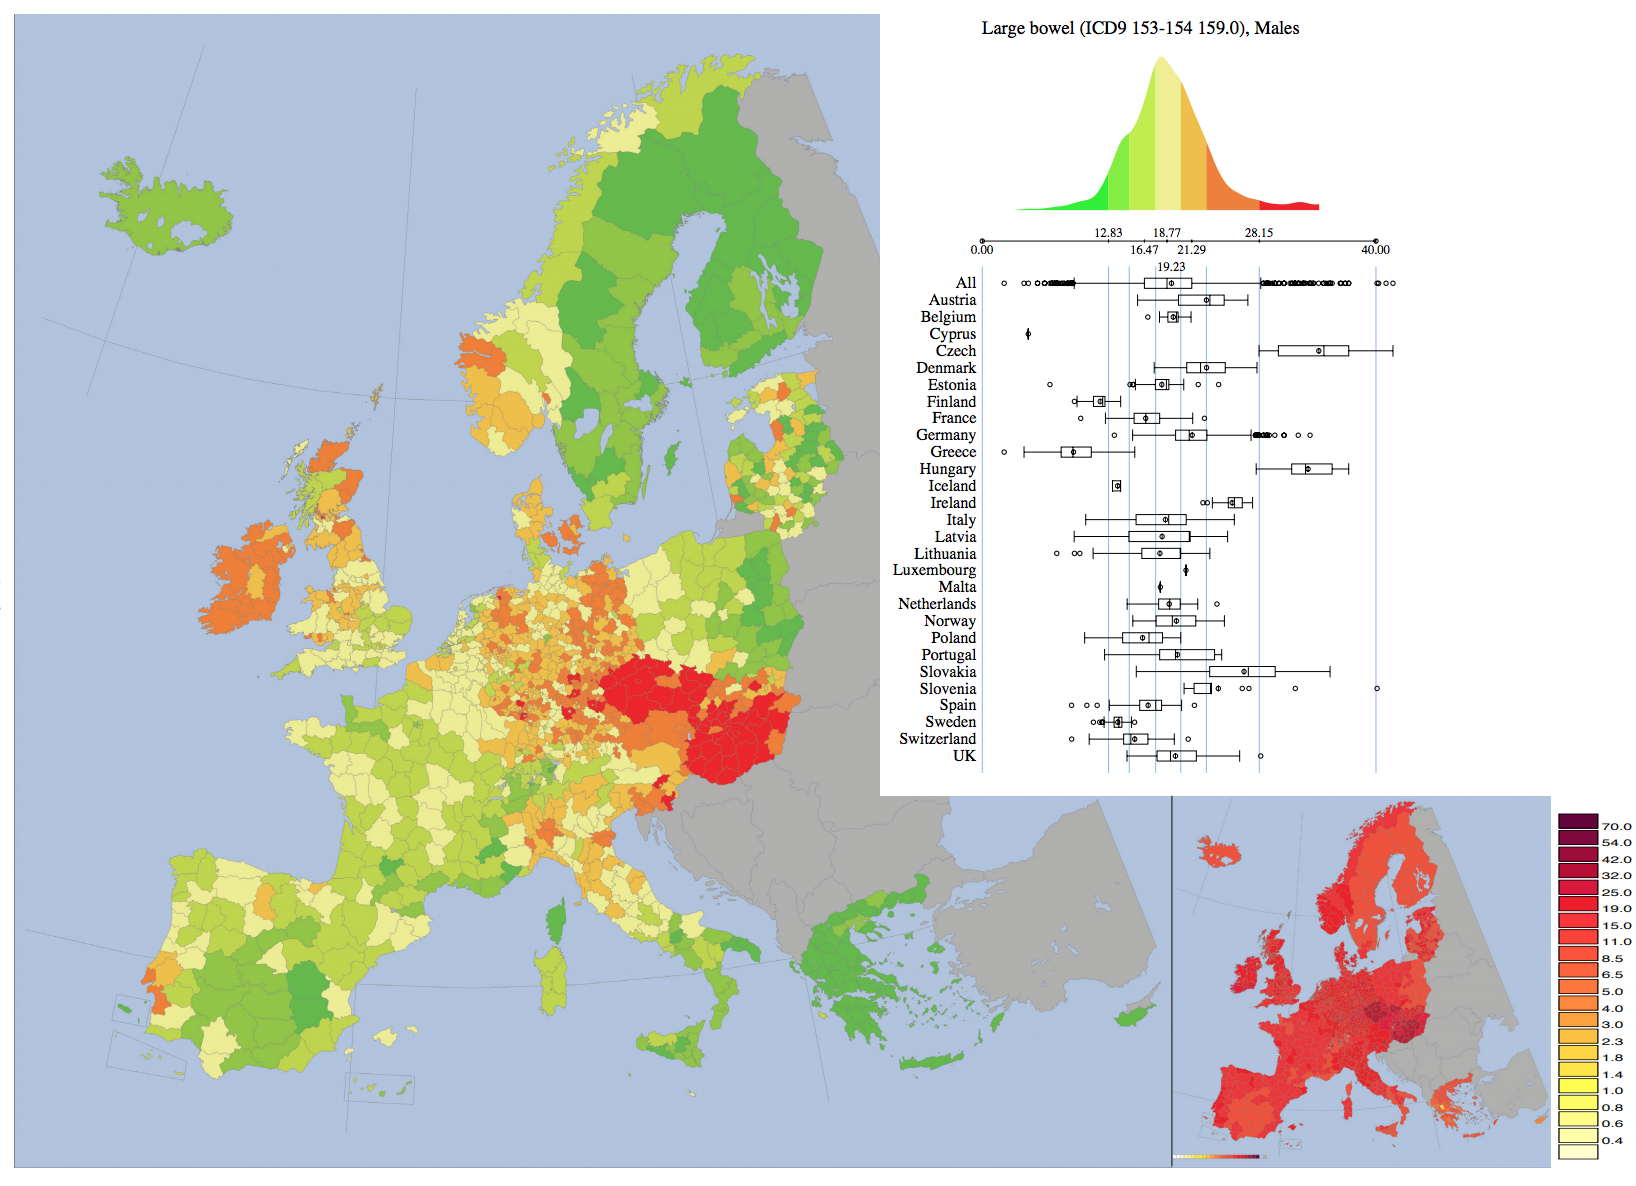
\includegraphics[width=0.9\linewidth]{figures/standard_deviation_large} 

}

\caption{Example of standard deviation visualised in cancer mapping}\label{fig:stndvn-example}
\end{figure}

\begin{longtable}[]{@{}ll@{}}
\caption{(\#tab:method-exp) Implicit and explicit measures of
uncertainty.}\tabularnewline
\toprule
\begin{minipage}[b]{0.35\columnwidth}\raggedright
Measure\strut
\end{minipage} & \begin{minipage}[b]{0.59\columnwidth}\raggedright
Example\strut
\end{minipage}\tabularnewline
\midrule
\endfirsthead
\toprule
\begin{minipage}[b]{0.35\columnwidth}\raggedright
Measure\strut
\end{minipage} & \begin{minipage}[b]{0.59\columnwidth}\raggedright
Example\strut
\end{minipage}\tabularnewline
\midrule
\endhead
\begin{minipage}[t]{0.35\columnwidth}\raggedright
CI Interval\strut
\end{minipage} & \begin{minipage}[t]{0.59\columnwidth}\raggedright
Figures 3.1, 3.2, 3.3\strut
\end{minipage}\tabularnewline
\begin{minipage}[t]{0.35\columnwidth}\raggedright
Statistical Significance\strut
\end{minipage} & \begin{minipage}[t]{0.59\columnwidth}\raggedright
Textured overlay on top of coloured regions used to indicate statistical
significance\strut
\end{minipage}\tabularnewline
\begin{minipage}[t]{0.35\columnwidth}\raggedright
Distribution\strut
\end{minipage} & \begin{minipage}[t]{0.59\columnwidth}\raggedright
Figure 3.4\strut
\end{minipage}\tabularnewline
\begin{minipage}[t]{0.35\columnwidth}\raggedright
Boxplots\strut
\end{minipage} & \begin{minipage}[t]{0.59\columnwidth}\raggedright
Figures 3.4, 3.5\strut
\end{minipage}\tabularnewline
\begin{minipage}[t]{0.35\columnwidth}\raggedright
Sample Size\strut
\end{minipage} & \begin{minipage}[t]{0.59\columnwidth}\raggedright
Textured overlay or lack of colour on a region, was used to show regions
with small sample size\strut
\end{minipage}\tabularnewline
\begin{minipage}[t]{0.35\columnwidth}\raggedright
Standard deviation\strut
\end{minipage} & \begin{minipage}[t]{0.59\columnwidth}\raggedright
Figure 3.6 - the second map in the bottom right corner shows standard
deviation\strut
\end{minipage}\tabularnewline
\bottomrule
\end{longtable}

\hypertarget{cartograms-as-an-alternative-display}{%
\subsection{Cartograms as an alternative
display}\label{cartograms-as-an-alternative-display}}

A cartogram alters the map base with the intention of improving the
presentation of the statistic of interest. For a single variable of
interest, each map area is changed to emphasise the distribution by
representing the corresponding value, in comparison to the value of the
other areas (Dougenik, Chrisman, and Niemeyer
\protect\hyperlink{ref-ACCAC}{1985}).

Choropleths may be considered true topological maps, however, if the
land mass displayed covers enough of the globe, there must be a
transformation or distortion to display the land in 2D. The amount of
distortion is related to the distance covered by the landmass displayed
Tobler (\protect\hyperlink{ref-GAMP}{1963}). World map projections
reflect the frequent perspectives used to view the earth. Choropleth
maps will always be distorted if they cover enough of the globe, just as
photographs of the globe from space. Choropleth creation requires
choosing a map projection that shows a favourable distortion of the
geography for presenting the set of spatial information. Diagrams that
do not specify a projection can be considered to have some unknown
projection.

If the statistic presented on the map base relies on physical distance
and is influenced by the topology there is no transformation needed
beyond choosing a projection. The purposeful distortion of the map space
is beneficial when a uniform density of the map base is desired. When a
map base is transformed according to population density, population
becomes a uniformly distributed background for the statistic presented
(Berry, Morrill, and Tobler, \protect\hyperlink{ref-GOINO}{n.d.}).

\begin{figure}
\centering
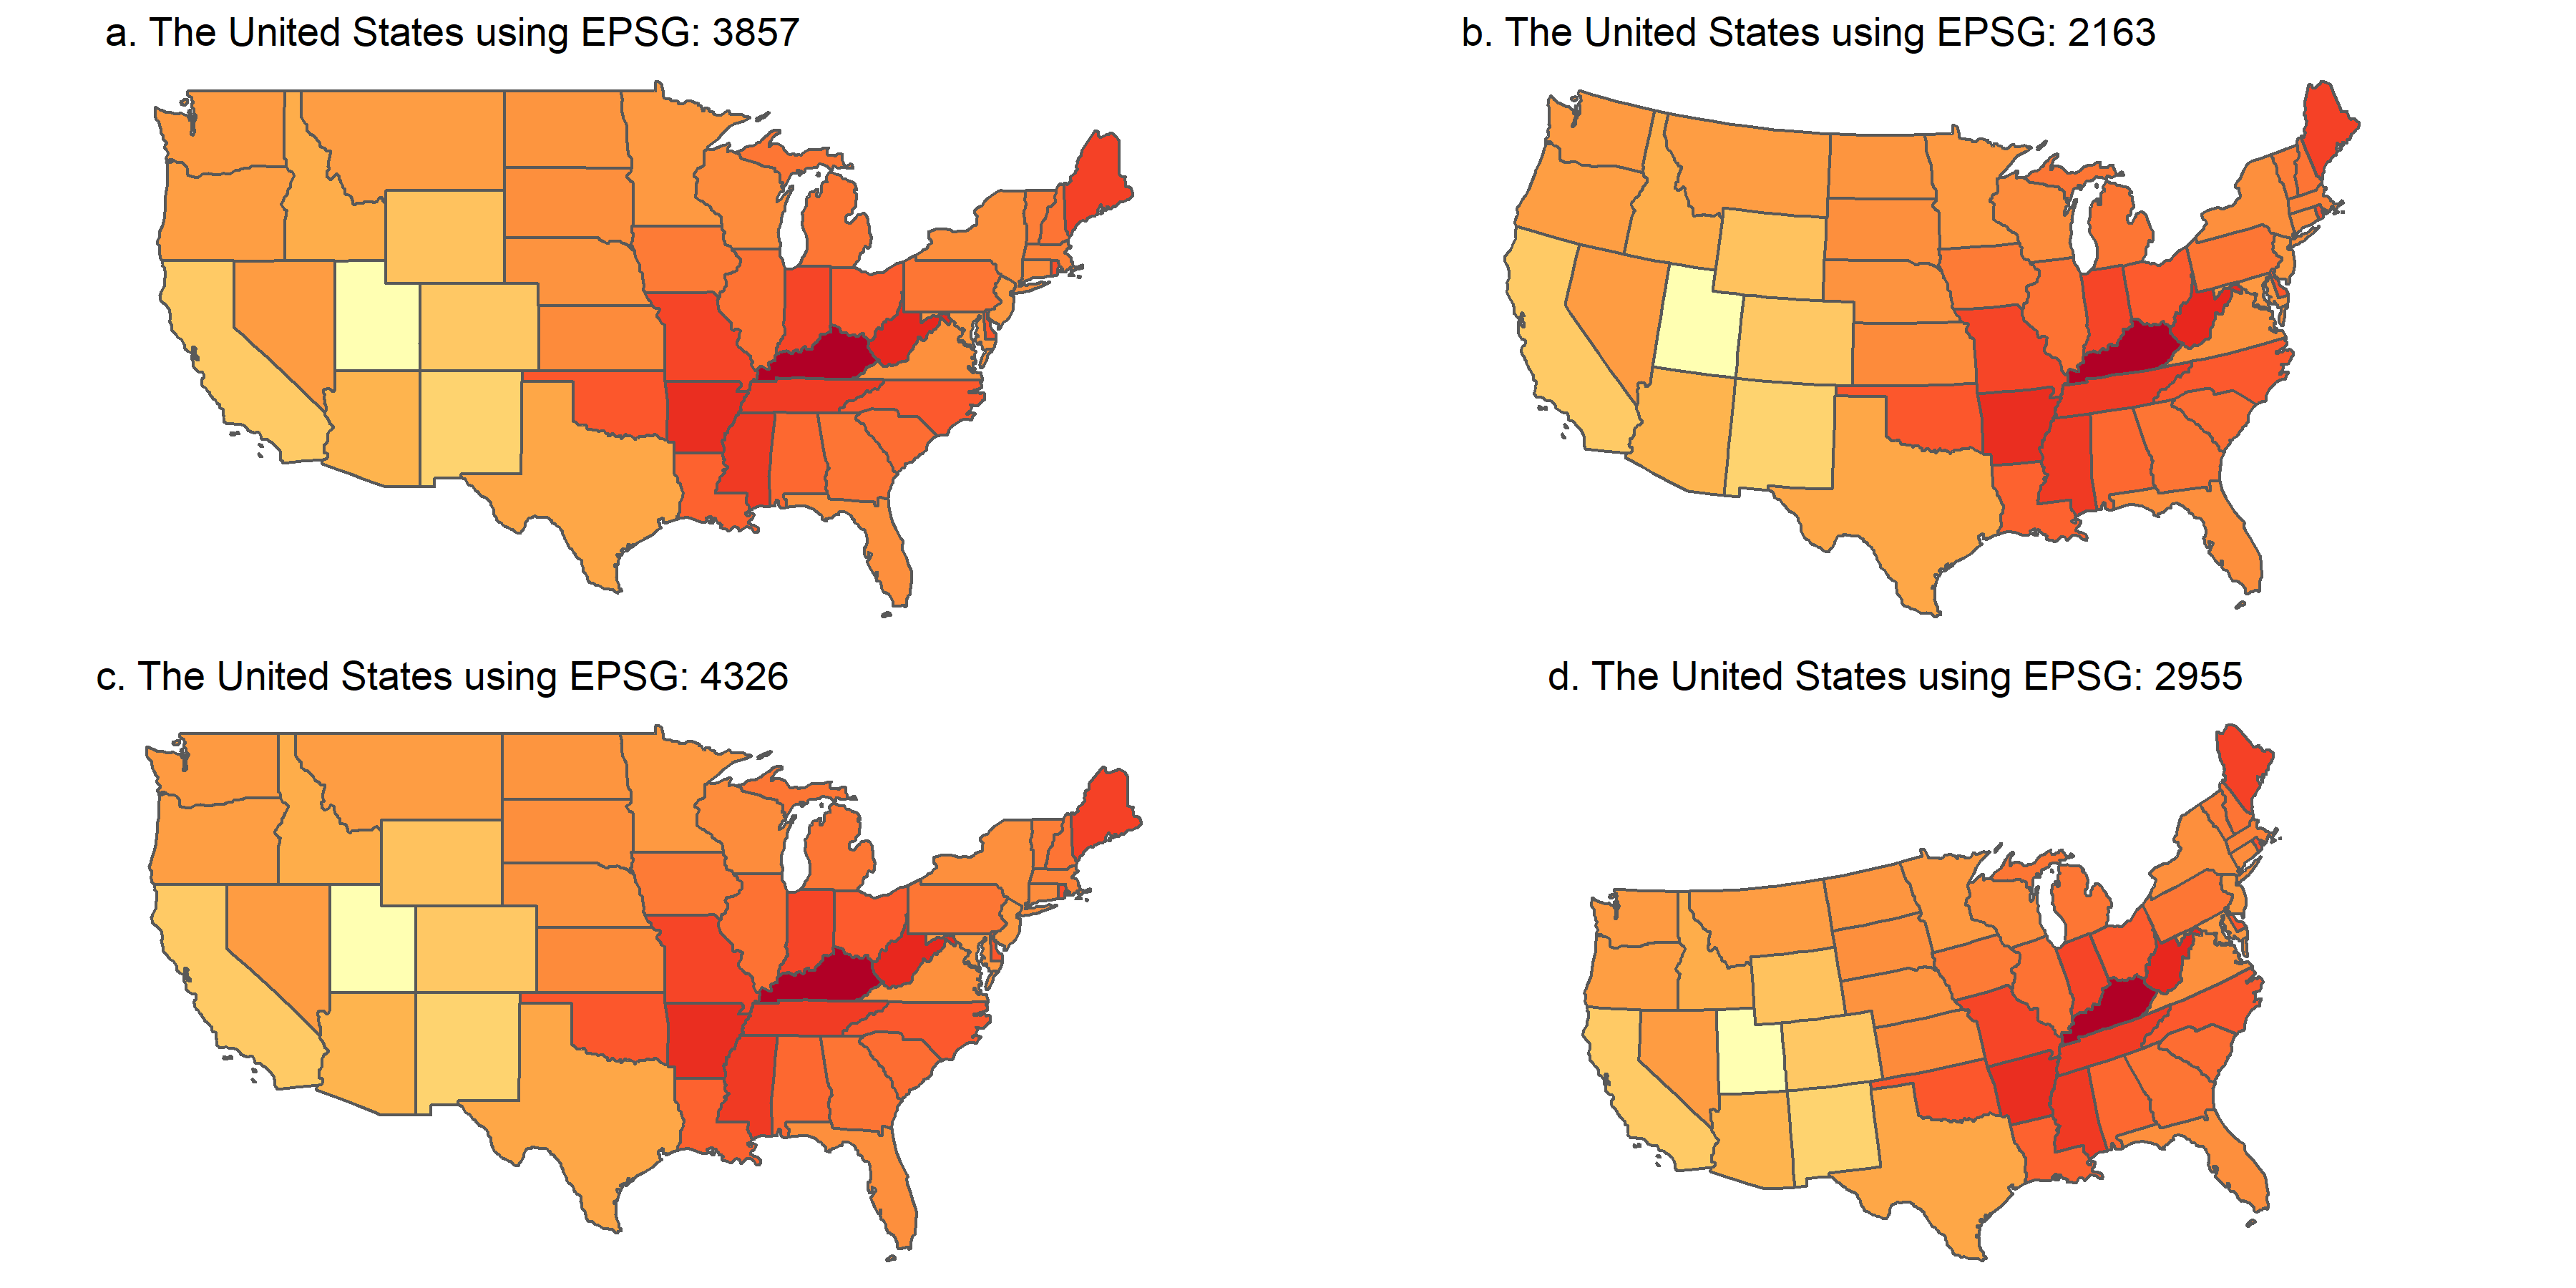
\includegraphics{figures/ggchoroCRS.png}
\caption{``Choropleth maps of the United States of America using four
coordinate reference systems.''}
\end{figure}

If the statistic presented on the map base relies on physical distance
and is influenced by the topology there is no transformation needed
beyond choosing a projection. The purposeful distortion of the map space
is beneficial when a uniform density of the map base is desired, Dorling
(\protect\hyperlink{ref-ACTUC}{2011}) suggests `population distribution
is often extremely uneven in former British colonies', this makes the
distortion necessary. When a map base is transformed according to
population density, population becomes a uniformly distributed
background for the statistic presented (Berry, Morrill, and Tobler,
\protect\hyperlink{ref-GOINO}{n.d.}). Using choropleth maps for
population characteristics requires graphic distortions when the
population concerned varies greatly in density (Griffin
\protect\hyperlink{ref-CTTMB}{1980}). When implementing a distortion of
the geographical shape according to population, an area cartogram (Olson
\protect\hyperlink{ref-NAC}{1976}), population-by-area cartograms
(Levison and Haddon Jr \protect\hyperlink{ref-TAAM}{1965}), or
iso-demographic map is the result.

Cartograms provide an alternative visualisation method for statistical
and geographical information. The key difference between a choropleth
and a cartogram is the desirable augmentation of the size, shape or
distance of geographical areas (Dorling
\protect\hyperlink{ref-ACTUC}{2011}). Cartograms may be seen as an
extension of map transformations and projections. The favourable
distortion is proportional to a value other other than actual earth size
area (Olson \protect\hyperlink{ref-NAC}{1976}). A disadvantage of the
conventional map is that sparsely populated rural areas may be
emphasized, whereas the areas representing cities are very small, making
interpretation of spatial patterns very difficult. The distortion of a
cartogram prevents the density obscuring the spatial patterns (Levison
and Haddon Jr \protect\hyperlink{ref-TAAM}{1965}). The spatial
transformation of map regions relative to the data emphasises the data
distribution instead of land size (Kocmoud and House
\protect\hyperlink{ref-CBATCC}{1998}). When visualising population
statistics Dorling (\protect\hyperlink{ref-ACTUC}{2011}) considers this
equitable representation design `more socially just', or honest (Dent
\protect\hyperlink{ref-NISCC}{1972}), giving due attention to all
members of the population and reducing the visual impact of large areas
with small populations (Walter \protect\hyperlink{ref-DMAHP}{2001}).
Griffin (\protect\hyperlink{ref-CTTMB}{1980}) suggest that spatial
socio-economic data is best presented on a cartogram for urban areas.
Howe (\protect\hyperlink{ref-HEDP}{1989}) agrees that `cancer occurs in
people, not in geographical areas' and the map bases of population
reflect this and avoid allocating `undue prominence' to rural areas.
Jahan et al. (\protect\hyperlink{ref-MTMSIH}{2018}) encourage the use of
cartograms to highlight small areas and uncover local-level
inequalities.

The creation of cartograms was largely in the hands of professional
cartographers (Kraak \protect\hyperlink{ref-CD}{2017}). Dorling
(\protect\hyperlink{ref-ACTUC}{2011}) discusses early approaches
including John Hunter and Jonathan Young (1968) and Durham's wooden tile
method, Skoda and Robertson's (1972) steel ball bearing approach and
Tobler's (1973) computer programs. Howe
(\protect\hyperlink{ref-HEDP}{1989}) discusses the impact of electronic
computer-assisted techniques. Geographical information systems allowed
map users, and researchers to implement their own cartograms, but these
systems are utilised depending on `the effectiveness, efficiency, and
satisfaction of the map products (Nielsen 1994)'(Kraak
\protect\hyperlink{ref-CD}{2017}).

There have been many algorithms presented, Nusrat and Kobourov
(\protect\hyperlink{ref-SAIC}{2016}) provided a framework to investigate
implementations and the ``statistical accuracy, geographical accuracy,
and topological accuracy''.

There are many alternatives to consider, the intended audience of the
map, and its purpose are key points in cartogram use and creation.
Dorling (\protect\hyperlink{ref-ACTUC}{2011}) reiterates: `There is no
``best'' cartogram or method of creating cartograms just as there is no
``best'' map' (Monmonier and Schnell, 1988).

\hypertarget{contiguous}{%
\subsubsection{Contiguous}\label{contiguous}}

\begin{figure}
\centering
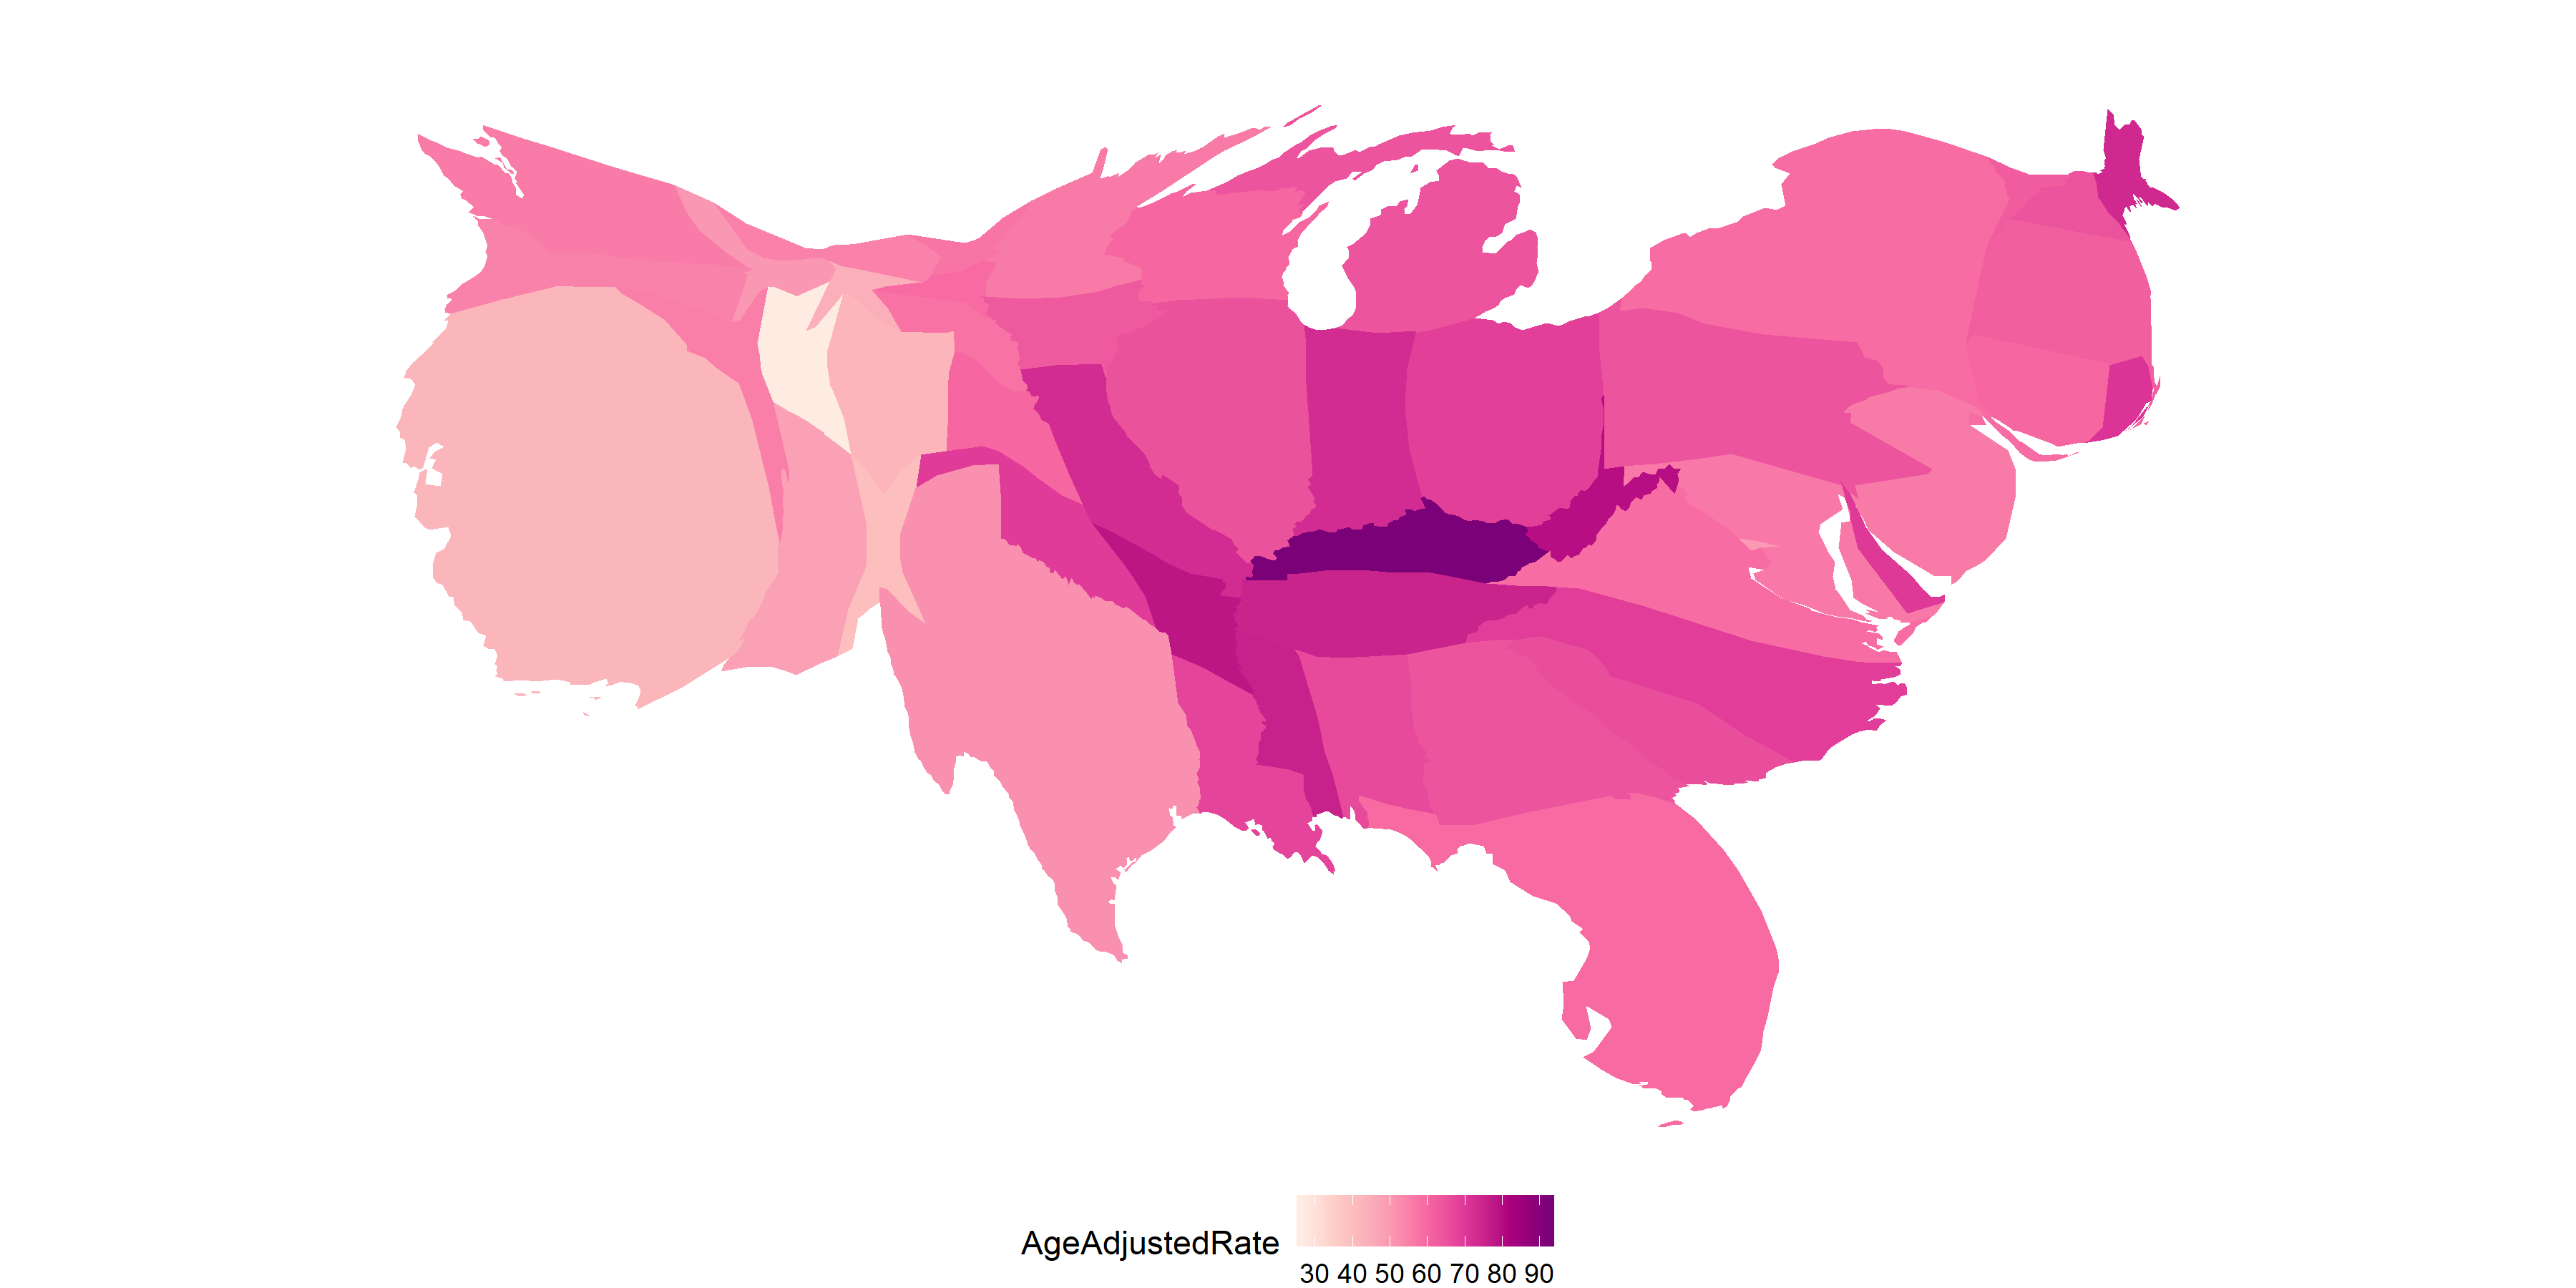
\includegraphics{figures/ggcont.png}
\caption{``A contiguous cartogram of the Unites States of America''}
\end{figure}

A contiguous cartogram maintains connectivity of the map regions while
areas are resized according to a statistic. This transformation often
occurs at the expense of the shape of areas (Kocmoud and House
\protect\hyperlink{ref-CBATCC}{1998}, @NAC, @TAAM). From a computer
graphics perspective, Min Ouyang and Revesz
(\protect\hyperlink{ref-ACA}{2000}) believe it is a problem of `map
deformation' to account for the value assigned to each area, they
provide three methods for creating value-by-area cartograms. Examples
include Tobler's Pseudo-Cartogram Method, Dorling's Cellular Automaton
Method (\protect\hyperlink{ref-ACTUC}{2011}), Radial Expansion Method of
Selvin et al., Rubber Sheet Method of Dougenik et al., Gusein-Zade and
Tikunov's Line Integral Method, Constraint-Based Method (Kocmoud and
House) (\protect\hyperlink{ref-CBATCC}{1998}).

An intentional goal when creating the 1966 Census population cartogram
for Canada was to maintain contiguity, while attempting to keep the
actual shape of places. The end result was a `very accurate
isodemo-graphic map of Canada'. This intentional design goal coincided
with the rising interest in urban geography.

To be able to recognise the significant changes, a reader will usually
have to know the initial geography to find the differences in the new
cartogram layout (Olson \protect\hyperlink{ref-NAC}{1976}). Tobler's
Conformal mapping means to preserve angles locally so that the shapes of
very small areas on a traditional map and a cartogram would be similar.
Kocmoud and House (\protect\hyperlink{ref-CBATCC}{1998}) presents this
issue as conflicting tasks or aims, to adjust region sizes and retain
region shapes. Distortion of region shapes on the contiguous cartogram
presents an additional hurdle to visual recognition and this hurdle is
not only eliminated on the noncontiguous cartogram but is replaced by
the meaningful empty-space property (Olson
\protect\hyperlink{ref-NAC}{1976}, @ECGC).

\hypertarget{non-contiguous}{%
\subsubsection{Non-Contiguous}\label{non-contiguous}}

\begin{figure}
\centering
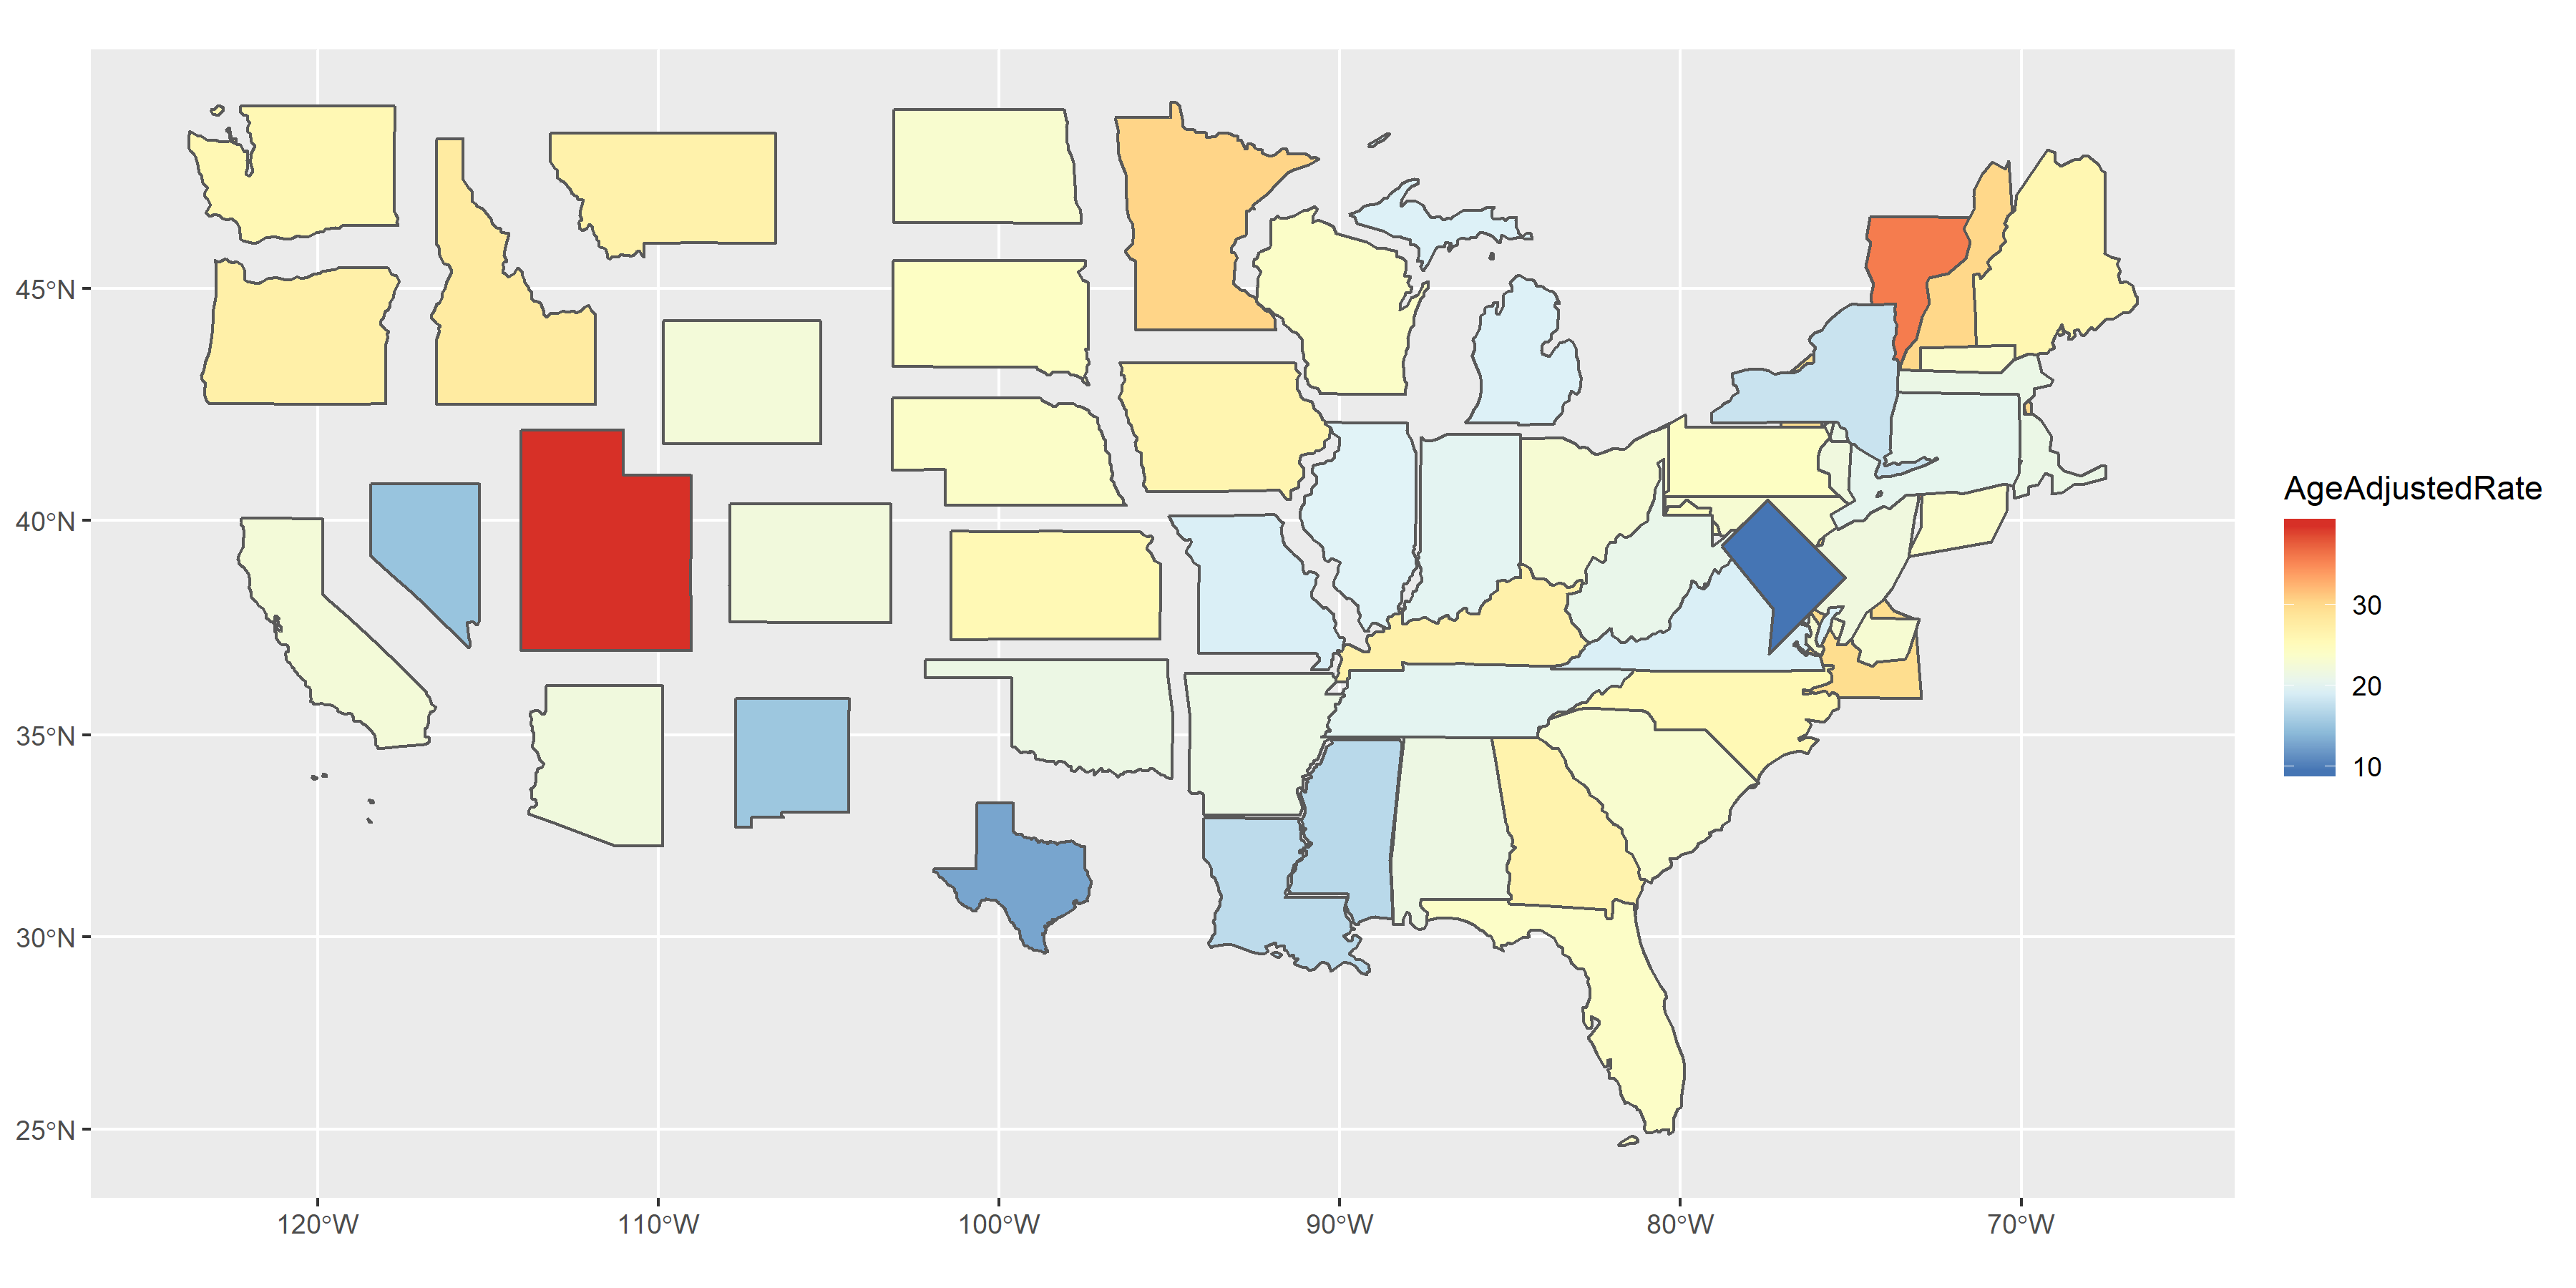
\includegraphics{figures/ggncont.png}
\caption{``A Non - contiguous cartogram of the Unites States of
America''}
\end{figure}

\begin{figure}
\centering
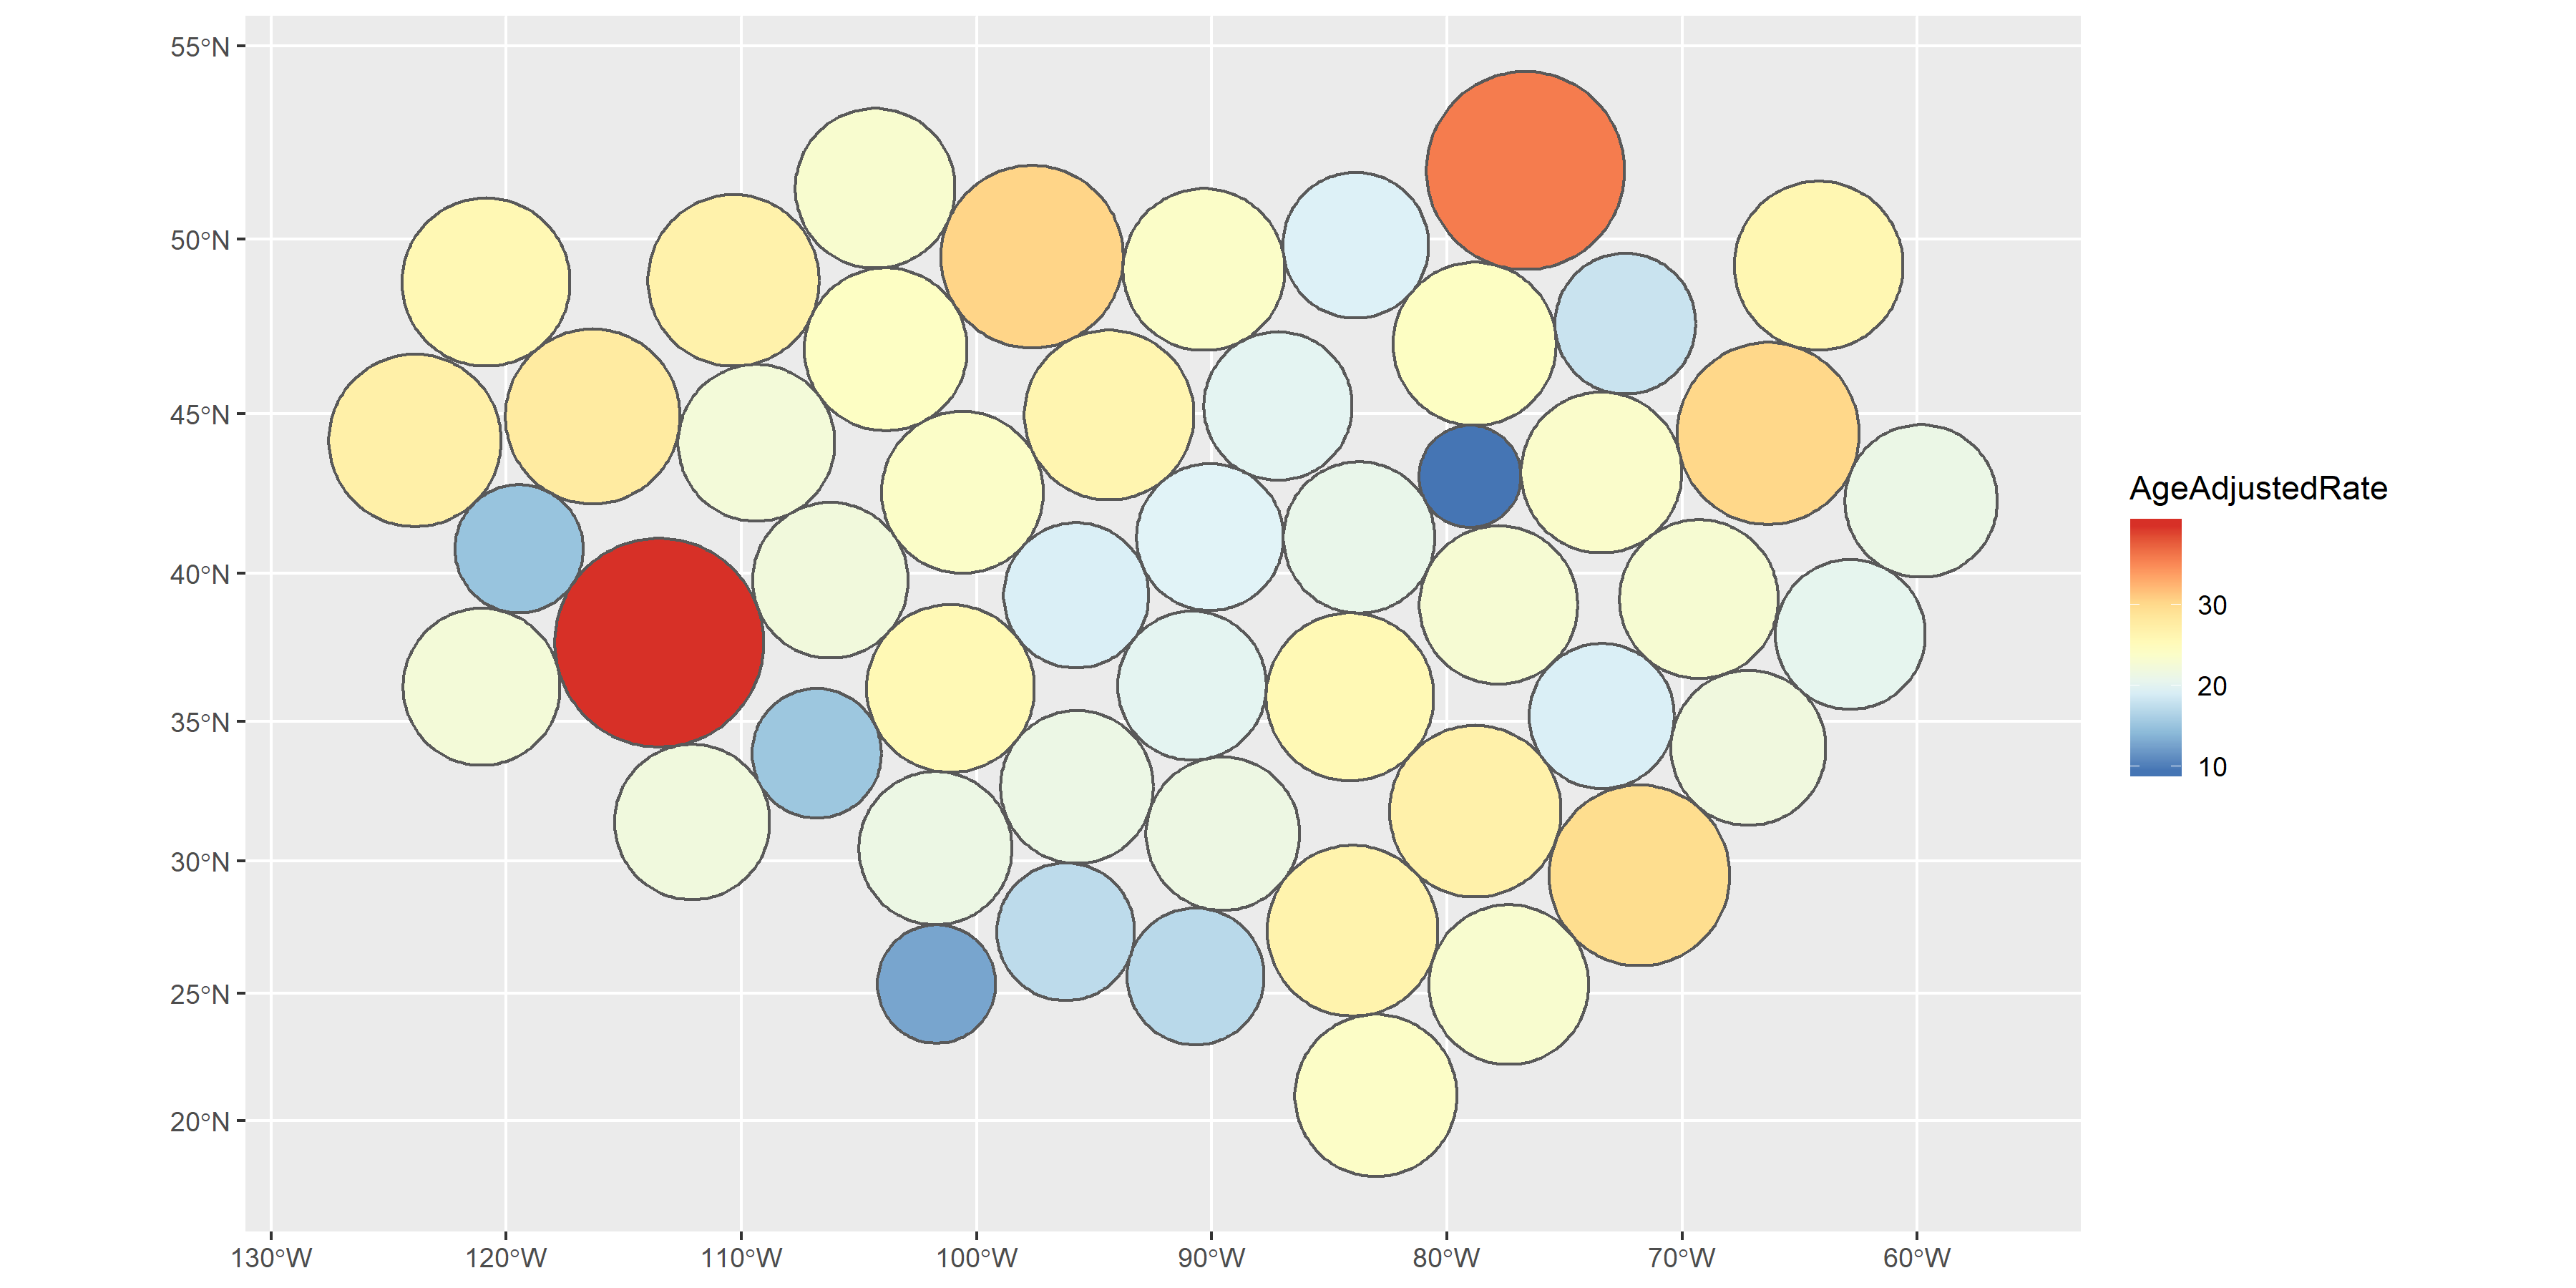
\includegraphics{figures/ggdorl.png}
\caption{``A dorling cartogram of the Unites States of America''}
\end{figure}

Dorling (\protect\hyperlink{ref-ACTUC}{2011}) puts forward a simple
question:

\begin{quote}
``If, for instance, it is desirable that areas on a map have boundaries
which are as simple as possible, why not draw the areas as simple shapes
in the first place?''
\end{quote}

He answers this with his implementation of maps created with `the
simplest of all shapes'. While contiguous cartograms may be a `more
sophisticated' method, they produce `very complex shapes'. Circular
cartograms use the same shape for every region represented, and size
them according to the statistic represented or the population for a base
map. To produce a compelling map, a gravity model is applied to avoid
overlaps, and keep spatial relationships with neighbouring areas over
many iterations. This implementation can work for up to `one hundred
thousand' areas.

`In Australia the urban federal constituencies occupy only a tenth of
the land, but contain nine tenths of the people. It would be almost
unthinkable to show election results for that country on a conventional
equal land area map.' This 1966 cartogram uses mostly straight lines,
and the result looks very little like the geographical shape of
Australia.

`Given the increasingly uneven population distribution of the United
States and the growing social divides between the populations of
neighbourhoods living at different densities, the need for cartograms
like this is greater now than ever.'

Used in displays of the UK by Howe in 1986 cited by Howe
(\protect\hyperlink{ref-HEDP}{1989})

Tobler's method and the many implementations that `elaborated' on it are
derived from `numerical approximations to a pair of equations'(Dorling
\protect\hyperlink{ref-ACTUC}{2011}). They all operate through
incremental adjustments, and can produce wildly different outcomes from
small changes in the inputs.

Tobler (\protect\hyperlink{ref-TFYCC}{2004}) Value-Area Cartograms. In
these cartograms a region,country, or continent is subdivided into small
regions, each of which is represented by a rectangle. This rectangle is
proportionate in area to the value which it represents in certain
statistical distributions. The regions are grouped in approximately the
same positions as they are on the map.

Computer generated map examples: Howe
(\protect\hyperlink{ref-HEDP}{1989}) (Hopps et al.~1968; Armstrong
1972). There has followed a flood of disease atlases, mainly
concentrating on the modem problems of cancer and degenerative diseases
from countries as scattered as the United States (Burbank 1971; Mason et
al.~1975, 1976; Pickle et al.~1987), the Soviet Union (Levin 1980),
Japan (Shigematsu 1977), the Federal Republic of Germany

Cano et al. (\protect\hyperlink{ref-MDAC}{2015}) define the term `mosaic
cartograms'. Compare amount of tiles to contrast population of regions.
`Cartograms show a data value per input region by scaling each region
such that its area is proportional to its data value. Mosaic cartograms
show data in multiples of tiles, hence the input data must consist of,
or be cast into, small integer units.'

\hypertarget{a-critique-of-mapping-methods}{%
\section{A critique of mapping
methods}\label{a-critique-of-mapping-methods}}

\begin{quote}
``designing a map tailored to precise goals {[}is{]} easier than forcing
a single map to accommodate diverse objectives'' Bell et al.
(\protect\hyperlink{ref-CPISACA}{2006})
\end{quote}

Waldo Tobler (\protect\hyperlink{ref-TVSSS}{2012}) explores many
graphical techniques, and suggests there are particular methods for
particular purposes. To choose an approporiate map display, the map
creator must consider the intended user, and message the map will
communicate. It is the objectives of the investigator that will drive
the choice of representation (Bell et al.
\protect\hyperlink{ref-CPISACA}{2006}).

There are two keys presented by Moore and Carpenter
(\protect\hyperlink{ref-SAMGIS}{1999}) to drive the choice of display: -
the properties of the visualisation, and - the ease or accuracy of
information extraction for map users

\hypertarget{animation-and-interactivity}{%
\section{Animation and
Interactivity}\label{animation-and-interactivity}}

Recent developments in technology allowed interactive web atlases.

\begin{quote}
``Where control of the message is important, static maps will continue
to be the most effective, although good tables, graphs, and explanatory
text are still needed in order to ensure that different people will see
the same thing in the maps'' Bell et al.
(\protect\hyperlink{ref-CPISACA}{2006})
\end{quote}

The intention of interactivity and animation is to allow users to answer
their own questions.

\hypertarget{acknowledgements}{%
\section{Acknowledgements}\label{acknowledgements}}

\hypertarget{references}{%
\section{References}\label{references}}

Wickham (\protect\hyperlink{ref-tidyerse}{2017}) for data analysis,
Bivand, Nowosad, and Lovelace (\protect\hyperlink{ref-spData}{2019}) and
Pebesma (\protect\hyperlink{ref-sf}{2018}) to implement plotting of
spatial data. Kobakian and Cook (\protect\hyperlink{ref-sugarbag}{2019})
to create hexagon tesselation. Arnold
(\protect\hyperlink{ref-ggthemes}{2019}) to enhance plot displays.
Jeworutzki (\protect\hyperlink{ref-cartogram}{2018}) for contiguous and
non-contiguous cartogram displays.

\hypertarget{refs}{}
\leavevmode\hypertarget{ref-ggthemes}{}%
Arnold, Jeffrey B. 2019. \emph{Ggthemes: Extra Themes, Scales and Geoms
for 'Ggplot2'}. \url{https://CRAN.R-project.org/package=ggthemes}.

\leavevmode\hypertarget{ref-CPISACA}{}%
Bell, B Sue, Richard E Hoskins, Linda Williams Pickle, and Daniel
Wartenberg. 2006. ``Current Practices in Spatial Analysis of Cancer
Data: Mapping Health Statistics to Inform Policymakers and the Public.''
\emph{International Journal of Health Geographics} 5: 49.
\url{https://doi.org/10.1186/1476-072X-5-49}.

\leavevmode\hypertarget{ref-GOINO}{}%
Berry, Brian J. L., Richard L. Morrill, and Waldo R. Tobler. n.d.
``GEOGRAPHIC Ordering of Information: NEW Opportunities'' 16 (4):
39--44. \url{https://doi.org/10.1111/j.0033-0124.1964.039_q.x}.

\leavevmode\hypertarget{ref-spData}{}%
Bivand, Roger, Jakub Nowosad, and Robin Lovelace. 2019. \emph{SpData:
Datasets for Spatial Analysis}.
\url{https://CRAN.R-project.org/package=spData}.

\leavevmode\hypertarget{ref-CIBMUK}{}%
Brewster, Mark B., and S. V. Subramanian. 2010. ``Cartographic Insights
into the Burden of Mortality in the United Kingdom: A Review of `The
Grim Reaper's Road Map'.'' Journal Article. \emph{International Journal
of Epidemiology} 39 (4): 1120--2.
\url{https://doi.org/10.1093/ije/dyp395}.

\leavevmode\hypertarget{ref-MDAC}{}%
Cano, R. G., K. Buchin, T. Castermans, A. Pieterse, W. Sonke, and B.
Speckmann. 2015. ``Mosaic Drawings and Cartograms.'' \emph{Computer
Graphics Forum} 34 (3): 361--70.

\leavevmode\hypertarget{ref-NISCC}{}%
Dent, Borden D. 1972. ``A Note on the Importance of Shape in Cartogram
Communication.'' \emph{Journal of Geography} 71 (7): 393--401.
\url{https://doi.org/10.1080/00221347208981697}.

\leavevmode\hypertarget{ref-MACM}{}%
d'Onofrio, Alberto, Chiara Mazzetta, Chris Robertson, Michel Smans,
Peter Boyle, and Mathieu Boniol. 2016. ``Maps and Atlases of Cancer
Mortality: A Review of a Useful Tool to Trigger New Questions.'' Journal
Article. \emph{Ecancermedicalscience} 10: 670--70.
\url{https://doi.org/10.3332/ecancer.2016.670}.

\leavevmode\hypertarget{ref-ACTUC}{}%
Dorling, Daniel. 2011. ``Area Cartograms: Their Use and Creation.'' In
\emph{Concepts and Techniques in Modern Geography (CATMOG)}, 59:252--60.
\url{https://doi.org/10.1002/9780470979587.ch33}.

\leavevmode\hypertarget{ref-TVSSS}{}%
---------. 2012. \emph{The Visualisation of Spatial Social Structure}.
John Wiley \& Sons Ltd.

\leavevmode\hypertarget{ref-ACCAC}{}%
Dougenik, James A., Nicholas R. Chrisman, and Duane R. Niemeyer. 1985.
``AN Algorithm to Construct Continuous Area Cartograms.'' \emph{The
Professional Geographer} 37 (1): 75--81.
\url{https://doi.org/10.1111/j.0033-0124.1985.00075.x}.

\leavevmode\hypertarget{ref-SE}{}%
Exeter, Daniel J. 2017. ``Spatial Epidemiology.'' Journal Article, 1--4.
\url{https://doi.org/10.1002/9781118786352.wbieg0283}.

\leavevmode\hypertarget{ref-CTTMB}{}%
Griffin, T.L.C. 1980. ``Cartographic Transformation of the Thematic Map
Base.'' \emph{Cartography} 11 (3): 163--74.
\url{https://doi.org/10.1080/00690805.1980.10438102}.

\leavevmode\hypertarget{ref-HEDP}{}%
Howe, G. M. 1989. ``Historical Evolution of Disease Mapping in General
and Specifically of Cancer Mapping.'' In \emph{Cancer Mapping}, edited
by Peter Boyle, Calum S. Muir, and Ekkehard Grundmann, 1--21. Berlin,
Heidelberg: Springer Berlin Heidelberg.

\leavevmode\hypertarget{ref-MTMSIH}{}%
Jahan, Farzana, Earl Duncan, Susanna Cramb, Peter Baade, and Kerrie
Mengersen. 2018. ``Making More of Spatial Maps: A Bayesian Meta-Analysis
Approach.'' In.

\leavevmode\hypertarget{ref-cartogram}{}%
Jeworutzki, Sebastian. 2018. \emph{Cartogram: Create Cartograms with R}.
\url{https://CRAN.R-project.org/package=cartogram}.

\leavevmode\hypertarget{ref-ECGC}{}%
Keim, D.A, S.C North, C Panse, and J Schneidewind. 2002. ``Efficient
Cartogram Generation: A Comparison.'' In \emph{IEEE Symposium on
Information Visualization, 2002. INFOVIS 2002}, 2002-:33--36. IEEE.

\leavevmode\hypertarget{ref-sugarbag}{}%
Kobakian, Stephanie, and Dianne Cook. 2019. \emph{Sugarbag: Create
Tessellated Hexagon Maps}.
\url{https://CRAN.R-project.org/package=sugarbag}.

\leavevmode\hypertarget{ref-CBATCC}{}%
Kocmoud, Christopher J., and Donald H. House. 1998. ``A Constraint-Based
Approach to Constructing Continuous Cartograms.'' In.

\leavevmode\hypertarget{ref-CD}{}%
Kraak, M. J. 2017. ``Cartographic Design.'' In \emph{The International
Encyclopedia of Geography : People, the Earth, Environment, and
Technology}, edited by D. Richardson, 1--16. United States: Wiley.

\leavevmode\hypertarget{ref-TAAM}{}%
Levison, M. E., and W. Haddon Jr. 1965. ``THE Area Adjusted Map. AN
Epidemiologic Device.'' Journal Article. \emph{Public Health Reports}
80: 55--59.

\leavevmode\hypertarget{ref-ACA}{}%
Min Ouyang, and P. Revesz. 2000. ``Algorithms for Cartogram Animation.''
In \emph{Proceedings 2000 International Database Engineering and
Applications Symposium (Cat. No.PR00789)}, 231--35.
\url{https://doi.org/10.1109/IDEAS.2000.880581}.

\leavevmode\hypertarget{ref-SAMGIS}{}%
Moore, Dale A., and Tim E. Carpenter. 1999. ``Spatial Analytical Methods
and Geographic Information Systems: Use in Health Research and
Epidemiology.'' \emph{Epidemiologic Reviews} 21 (2): 143--61.
\url{https://doi.org/10.1093/oxfordjournals.epirev.a017993}.

\leavevmode\hypertarget{ref-SAIC}{}%
Nusrat, Sabrina, and Stephen G. Kobourov. 2016. ``The State of the Art
in Cartograms.'' \emph{CoRR} abs/1605.08485.
\url{http://arxiv.org/abs/1605.08485}.

\leavevmode\hypertarget{ref-NAC}{}%
Olson, Judy M. 1976. ``NONCONTIGUOUS Area Cartograms.'' \emph{The
Professional Geographer} 28 (4): 371--80.
\url{https://doi.org/10.1111/j.0033-0124.1976.00371.x}.

\leavevmode\hypertarget{ref-sf}{}%
Pebesma, Edzer. 2018. ``Simple Features for R: Standardized Support for
Spatial Vector Data.'' \emph{The R Journal} 10 (1): 439--46.
\url{https://doi.org/10.32614/RJ-2018-009}.

\leavevmode\hypertarget{ref-GAMP}{}%
Tobler, Waldo. 1963. ``Geographic Area and Map Projections,'' January,
59--78. \url{https://www.jstor.org/stable/212809}.

\leavevmode\hypertarget{ref-TFYCC}{}%
---------. 2004. ``Thirty Five Years of Computer Cartograms.''
\emph{Annals of the Association of American Geographers} 94 (1): 58--73.

\leavevmode\hypertarget{ref-EI}{}%
Tufte, Edward R. 1990. \emph{Envisioning Information}. Graphics Press.

\leavevmode\hypertarget{ref-DMAHP}{}%
Walter, S. D. 2001. \emph{Disease Mapping: A Historical Perspective}.
Book. Oxford University Press: Oxford.

\leavevmode\hypertarget{ref-tidyerse}{}%
Wickham, Hadley. 2017. \emph{Tidyverse: Easily Install and Load the
'Tidyverse'}. \url{https://CRAN.R-project.org/package=tidyverse}.


\end{document}
